\documentclass[11pt]{article}
\usepackage{amssymb}
\usepackage[english]{babel}
\usepackage{fullpage}
\usepackage{graphicx}
\def\titre{}
\def\auteur{}
\def\courriel{}
\makeatletter

\title{LOG8415\\Advanced Concepts of Cloud Computing\\Lab 2}

\author{
    Amin Nikanjam \\
    D\'{e}partement G\'{e}nie Informatique et G\'{e}nie Logiciel \\
    \'{E}cole Polytechnique de Montr\'{e}al, Qu\'{e}bec, Canada \\
    \texttt{amin.nikanjam[at]polymtl.ca} \\
}

\date{}

\begin{document}
\maketitle

\section{Identification}

\paragraph{Students name:} 
\begin{itemize}
	\item Maximiliano Falicoff
	\item Corentin Glaus
	\item Aymeric Labrie
	\item William Trépanier

\end{itemize}
\auteur

\paragraph{Date of submission:} Saturday November 11^{th} \; 2023

\section{How we utilized docker}
Docker was used only for the machine learning (ML) applications deployed on the workers, the orchestrator didn't need it since it was the only service running in the VM. The docker images are built with a Dockerfile, which specifies the port that needs to be exposed for the flask server. The image is also made so that when the container is started, it will also start the flask server specified in the Dockerfile. 
\newline
\\
Since for every worker we need two containers, we use compose to start two containers of the image with the ML application with different port mapping.

\section{Our Orchestrator}
We decided to omit using a json based file to track our worker statutes and decide to use semaphores to implement our queue. We have a semaphore to keep track of the number of free containers that are available to precess new requests, along with this we setup a dictionary to map each container id to a lock, to know if a container is busy or not. We have a request queue that is initialized. Our route /new\_requests will enqueue the request to the queue. We defined a consume function that waits for a request from the queue and acquire a container (decrements the semaphore), it will then lock the container, starts a new thread to send the request to the container.
\newline
\\
Our function to send a request to a container sends the request to the container and then releases the lock on the container and increments the semaphore to indicate it is free.

\section{How we deployed our code}
We are using terraform to deploy our infrastructure. We have two security groups, one for our orchestrator and one for our workers. Only the orchestrator can communicate with the broad internet both ways (ingress and egress) whereas our worker can only communicate with our orchestrator in ingress, but the workers can return responses to the broad internet.
\newline
\\
We then have our ec2 instances, with one replica for our orchestrator and 5 replicas for our workers. Our orchestrator has a specific setup script where we do the same setup that we did in our lab 1, we echo our orchestrator app to a python file on our ec2 instance and install the requirements, create a virtual environment and finally create and start a system service running our flask server.
\newline
\\
In terms of our workers we do the same process but instead on running through a service we build.a docker image and use a docker compose stack to launch two instance of our server on two different ports 5000 and 5001

\section{Testing our deployment}

In order to test our deployment, we made a script that creates 5 threads, each sending 10 requests to our orchestrator. We can then ssh into the orchestrator and see in the logs how it handled the requests as it's setup as a service.


\section{Results}
Running our script we found that our orchestrator handles many requests as we wanted, it will use the 10 available containers by checking if there is a free container, if there is not, we will wait for the next iteration of our loop if there is a free container we forward the request.

Our machine running the requests script will receive a 200 OK from the orchestrator if the request was successfully enqueued


\begin{figure}[ht]
  \centering
  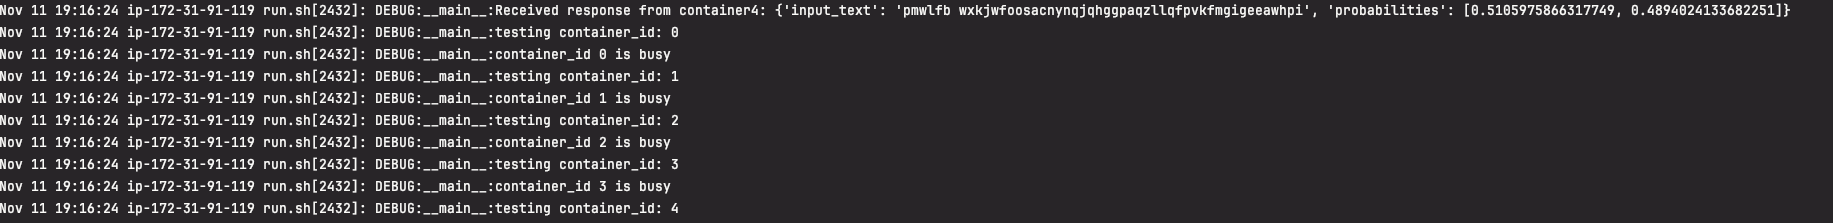
\includegraphics[width=\textwidth]{images/container_busy}
  \caption{How our Orchestrator handles requests}
  \label{fig:container_busy}
\end{figure}

\section{How to run our code}
Ensure the following packages are installed on the system
\begin{itemize}
	\item aws-cli
	\item terraform
	\item pv
\end{itemize}
\newline
Copy your aws credentials to ~/.aws/credentials, they should be in the following format:
\newline
[default] \newline
aws\_access\_key\_id=\_ \newline
aws\_secret\_access\_key=\_ \newline
aws\_session\_token=\_
\newline
\\
Make the script executable: chmod +x scripts.sh \newline
Then run the script: ./scripts.sh

\end{document}